\begin{figure}[htbp!]
 \centering
 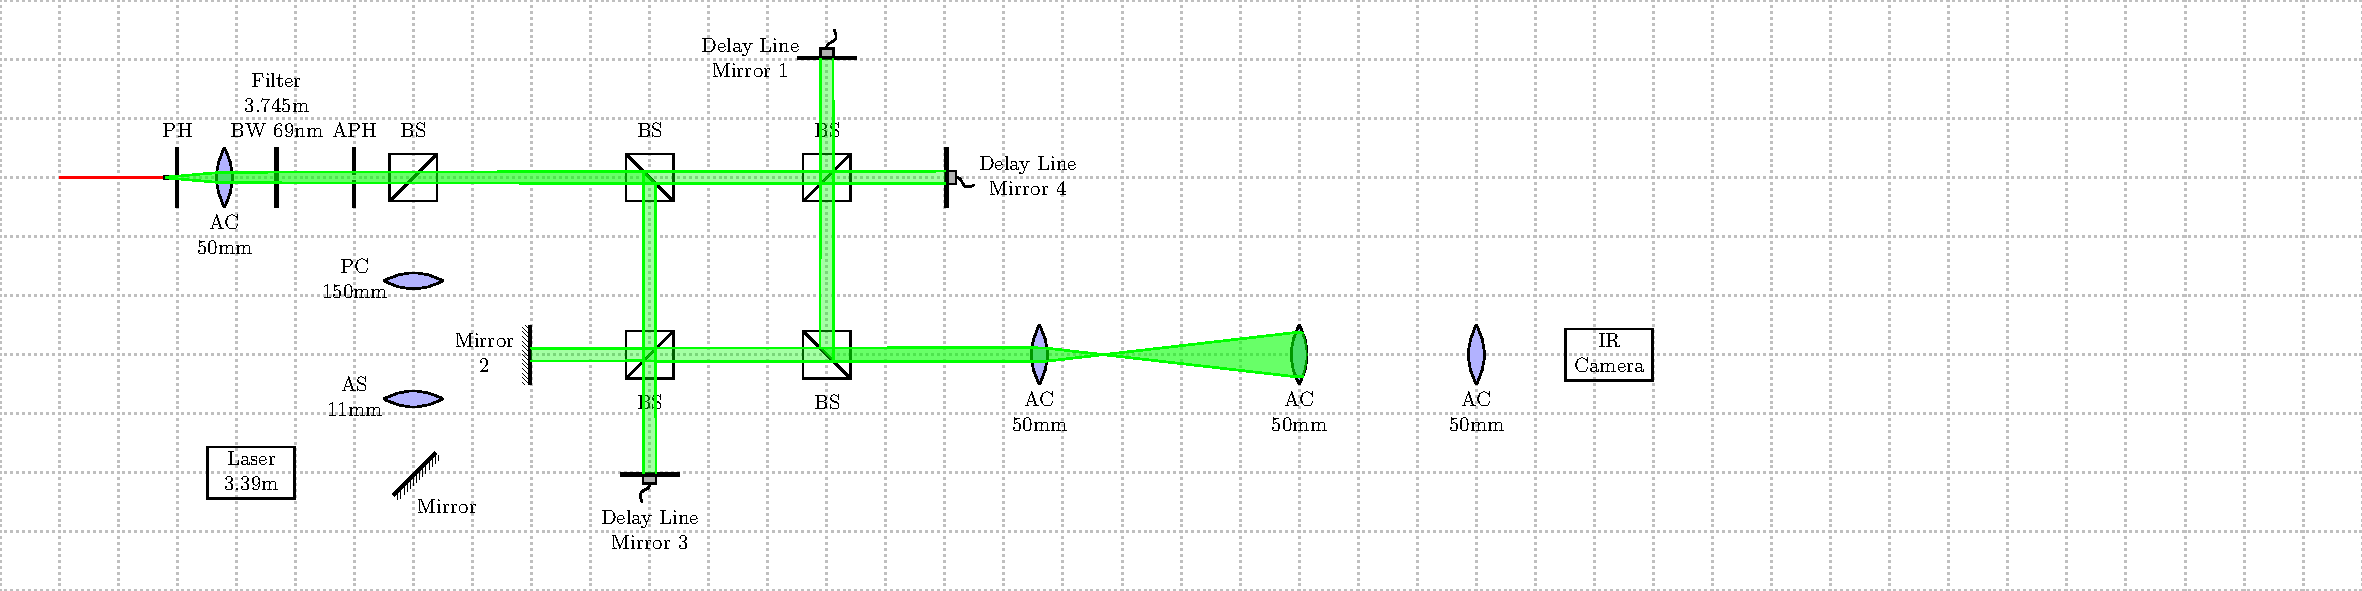
\includegraphics[scale=.53]{../figures/montage.pdf}
 \caption{Experimental setup for characterization of the ZigZag DBC integrated optics chip. The last two lens are used to magnify approximately 8 times. AC = Achromatic, AS = Asphere, PH = PinHole, APH = Adjustable PinHole, BS = Beam-Splitter, PC = Plano-Convex.}
 \label{fig:expersetup}
\end{figure}
 
It has been demonstrated in the previous section that the ZigZag DBC can give accurate results with a bandwidth up to 70nm. The purpose of this part is to verify that experimentally. 
For that purpose the experimental setup represented in Fig.\ref{fig:expersetup} was used. It is a Michelson interferometer with 4 beams. The beams from Mirror 1, 2, 3 and 4 are coupled in the input waveguides 5, 14, 10 and 19 respectively (see Fig \ref{tikz:ZigZagCrossSection} as seen from the input side). 

The DBC used for the characterization is not the one designed in the previous chapter, but is designed to word at 3.4\si{\micro\meter} too. Asit appear that at 3.4\si{\micro\meter} all outputs were not illuminated, the source signal was chosen to be a "flat" spectrum signal of 69nm bandwidth centered at 3.745\si{\micro\meter}. If the component was well inscribed in the glass all photometric signal should be symmetrical (i.e the ones from inputs 2,3 and 4,1 should look alike). As can be seen in Fig.\ref{fig:photometries} this is not the cas especially for inputs 4, 1. The reason of this is to be found in the writing technique. As the laser inscription technique is not the purpose of this report we will simply explain how it induce birefringence. To inscribe the waveguides the laser write multiple lines that overlap each-other. This overlapping lines make the result dependant of the order of inscription of the waveguides which cause the birefringence effect responsible of the not symmetrical pattern. This has to be verified using a polariser.

\begin{figure}
 \centering
 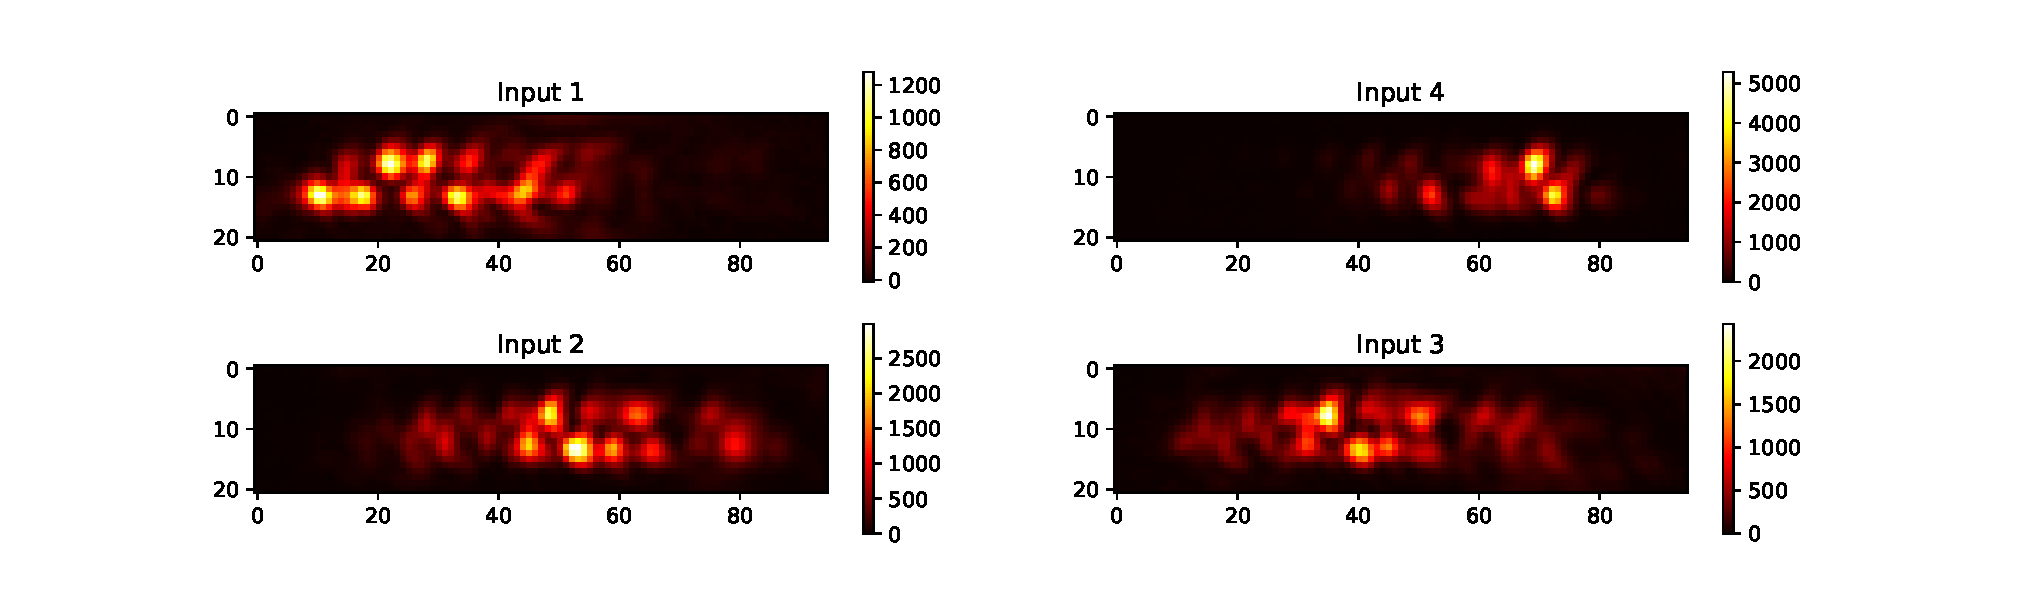
\includegraphics[scale=.45]{photometries.pdf}
 \caption{The photometric signal of the DBC. As can be seen the signal from input 4 ans 1 are not symmetrical certainly due to birefringence.}
 \label{fig:photometries}
\end{figure}

A second point to explain is the presence of the laser. As the Delay-lines were not very accurate in their mouvement, the laser was here to calibrate the OPD. Using the fringe spacing of the laser's interferogram, one can reconstruct the real OPD introduced by the delay-line. In order to do so in a First experiment the laser was coupled into the DBC together with the supercontinum source (at 3.8 \si{\micro\meter}). As it appeared that the laser signal was not enough distinguishable from the source signal this technique was not used to obtain the results presented in the following paragraph.  Rather than doing that, as the "apparent wavelength" of the high-frequency component of the interferogram has been demonstrated to be quite the same for all output at 70nm bandwidth, one interferogram was used to calibrate the OPD stating that the fringe spacing was 3.745\si{\micro\meter}. 

This method is valid in the limit of "apparent frequency" not too different from one output to the other. In fact this was verified as for BL-1/2 the apparent wavelength was $3.73\pm0.05\si{\micro\meter}$, $3.73\pm0.04\si{\micro\meter}$ for BL-1/3, $3.70\pm0.08\si{\micro\meter}$ for BL-1/4, $3.78\pm0.04\si{\micro\meter}$ for BL-2/3, $3.75\pm0.05\si{\micro\meter}$ for BL-2/4 and $3.69\pm0.07\si{\micro\meter}$ for BL-3/4. This is of the same order of magnitude than what was seen in simulation. 

In order to characterize the V2PM, the following measurements are performed for each of the 6 baselines (recording frequency = 100Hz, delay line velocity = 0.08 mm/s):
\begin{enumerate}
 \item Record the signal from the moving delay-line alone $I_{DL}$ with the delay-line moving (5000 frames).
 \item Record the photometry from the non-moving input alone $I_{Fix}$.
 \item Record the interferogram (with the 2 beams) $I$
\end{enumerate}

The obtained result is in the form of a cube of frames. In these frames 1 pixel is chosen to be approximately centered on each output in order to be influenced as little as possible by the surroundings waveguides (as explained in the first chapter. This pixel with the magnification system of 8 should be an area of less than $4\times 4 \si{\micro\meter}$ which was too large in simulation but the best doable at with the setup. - In the case of the component with fanout, one would have to integral all the flux by taking an area around the output in order to have high SNR - . Then the data is processed to build the V2PM as follows :
\begin{enumerate}
 \item The noise is filtered in Fourier's space.
 \item The OPD is calculated using a chosen interferogram stating that the fringe spacing which should be 3.745µm.
 \item $I_{DL}$ and $I_{Fix}$ are subtracted from the interferogram.
 \item The protocorrection is applied (Eq \ref{eq:photocorpoly})
 \item The envelop of the signal is fitted and the instrumental visibility deduced by it's amplitude
 \item A cosine is fitted to 3 fringes of the interferogram centered at the position of it's maximum to deduce the phase (being $2\pi x/\lambda_0$, $\lambda_0 = 3.745\si{\micro\meter} in our case$)
 \item the transmission coefficients of the input ($\kappa_{io}$ for input i to output o) are calculated from the photometric data (averaged along the number of frames) by $\kappa_{io} = \frac{I_D(o)}{\sum_{all\_pixels}{I_D(pixel)}}$
 \item The whole V2PM is calculated as in the case of monochromatic light
\end{enumerate}

The condition number of the V2PM resulting with the tested component (numbered 39.7) is 26. The instrumental visibilities for the majority range between 0.6 and 1 which is comparable to the results obtained in simulation. An histogram of the visibilities is shown in Fig.\ref{fig:hist}. 

\begin{figure}[htbp!]
 \centering
 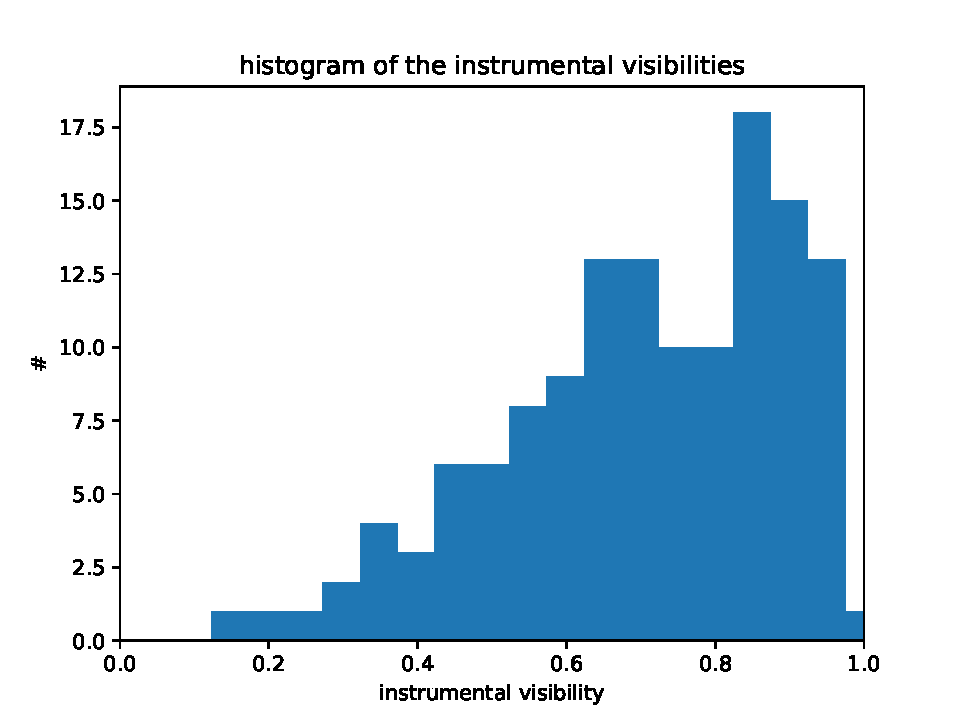
\includegraphics[scale=.5]{../picture/hist.pdf}
 \caption{Histogram of the instrumental visibilities of the ZigZag DBC number 39.7}
 \label{fig:hist}
\end{figure}


From that V2PM the visibilities and phases of each baselines are retrieved first using directly the data used to calibrate the V2PM, then using data recorded after with 2 or 4 beams in input. The results are presented in the next section. 


